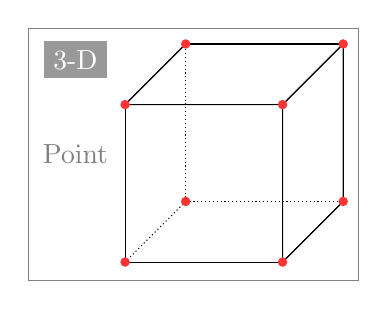
\begin{tikzpicture}
%draw the axes
% \draw[->] (0,0,0) -- (3,0,0) node[anchor=west]{$x$};
% \draw[->] (0,0,0) -- (0,3,0) node[anchor=west]{$y$};
% \draw[->] (0,0,0) -- (0,0,3) node[anchor=west]{$z$};

%draw the top and bottom of the cube
\draw[gray] (-2.0, -1) rectangle (2.2, 2.2);
\node[gray] (name) at (-1.4, 0.6) {Point};
\node[color=white, fill=gray!80] (name) at (-1.4, 1.8) {3-D};

\draw[] (2,0,0) -- (2,2,0) -- (2,2,2) -- (2,0,2) -- cycle;
\draw[] (0,0,2) -- (0,2,2) -- (2,2,2) -- (2,0,2) -- cycle;
\draw[] (0,2,0) -- (2,2,0) -- (2,2,2) -- (0,2,2) -- cycle;

\draw[] (0,2,2) -- (0,2,0);
\draw[] (2,0,0) -- (2,2,0);
\draw[] (2,0,0) -- (2,0,2);
\draw[] (2,0,2) -- (0,0,2);
\draw[] (0,0,2) -- (0,2,2);
\draw[] (0,2,0) -- (2,2,0);

%draw the edges of the cube
\draw[densely dotted] (0,0,0) -- (0,0,2);
\draw[densely dotted] (0,0,0) -- (0,2,0);
\draw[densely dotted] (0,0,0) -- (2,0,0);

\fill [red!80] (0, 2, 0) circle [radius=0.06cm];
\fill [red!80] (2, 2, 0) circle [radius=0.06cm];
\fill [red!80] (0, 2, 2) circle [radius=0.06cm];
\fill [red!80] (0, 0, 2) circle [radius=0.06cm];
\fill [red!80] (2, 0, 2) circle [radius=0.06cm];
\fill [red!80] (2, 0, 0) circle [radius=0.06cm];
\fill [red!80] (0, 0, 0) circle [radius=0.06cm];
\fill [red!80] (2, 2, 2) circle [radius=0.06cm];

\end{tikzpicture}